

\documentclass{article}
\usepackage[utf8]{inputenc}
\usepackage[utf8]{inputenc}
\usepackage[T1]{fontenc}
\usepackage[english]{babel}
\usepackage{fullpage}
\usepackage{color}
\usepackage[table]{xcolor}
\usepackage{listings}
 
\definecolor{darkWhite}{rgb}{0.94,0.94,0.94}
 
\lstset{
  aboveskip=3mm,
  belowskip=-2mm,
  backgroundcolor=\color{darkWhite},
  basicstyle=\footnotesize,
  breakatwhitespace=false,
  breaklines=true,
  captionpos=b,
  commentstyle=\color{red},
  deletekeywords={...},
  escapeinside={\%*}{*)},
  extendedchars=true,
  framexleftmargin=16pt,
  framextopmargin=3pt,
  framexbottommargin=6pt,
  frame=tb,
  keepspaces=true,
  keywordstyle=\color{blue},
  language=C,
  literate=
  {²}{{\textsuperscript{2}}}1
  {⁴}{{\textsuperscript{4}}}1
  {⁶}{{\textsuperscript{6}}}1
  {⁸}{{\textsuperscript{8}}}1
  {€}{{\euro{}}}1
  {é}{{\'e}}1
  {è}{{\`{e}}}1
  {ê}{{\^{e}}}1
  {ë}{{\¨{e}}}1
  {É}{{\'{E}}}1
  {Ê}{{\^{E}}}1
  {û}{{\^{u}}}1
  {ù}{{\`{u}}}1
  {â}{{\^{a}}}1
  {à}{{\`{a}}}1
  {á}{{\'{a}}}1
  {ã}{{\~{a}}}1
  {Á}{{\'{A}}}1
  {Â}{{\^{A}}}1
  {Ã}{{\~{A}}}1
  {ç}{{\c{c}}}1
  {Ç}{{\c{C}}}1
  {õ}{{\~{o}}}1
  {ó}{{\'{o}}}1
  {ô}{{\^{o}}}1
  {Õ}{{\~{O}}}1
  {Ó}{{\'{O}}}1
  {Ô}{{\^{O}}}1
  {î}{{\^{i}}}1
  {Î}{{\^{I}}}1
  {í}{{\'{i}}}1
  {Í}{{\~{Í}}}1,
  morekeywords={*,...},
  numbers=left,
  numbersep=10pt,
  numberstyle=\tiny\color{black},
  rulecolor=\color{black},
  showspaces=false,
  showstringspaces=false,
  showtabs=false,
  stepnumber=1,
  stringstyle=\color{gray},
  tabsize=4,
  title=\lstname,
}
\usepackage{graphicx}
\title{HAI804I – Codage et compression multimédia
}
\author{Fabien Caballero}

\begin{document}

\maketitle
    \tableofcontents

\newpage

\begin{figure}[h]
\centerline{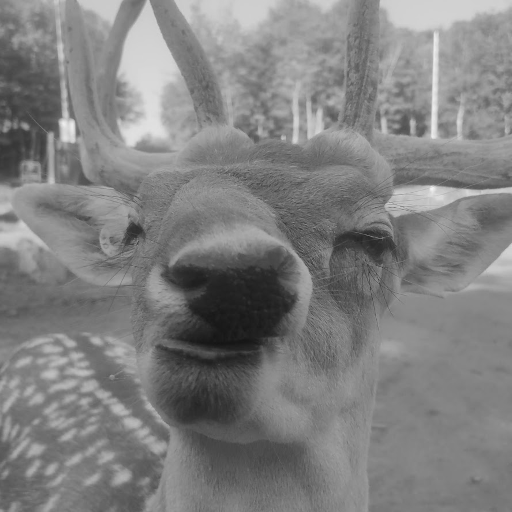
\includegraphics[scale=0.5]{./pierrelouis.png}}
\caption{pierre louis original}
\end{figure}

\addcontentsline{toc}{section}{Introduction}
\section*{Introduction}
L'objectif de ce TP est de comprendre la segmentation d’une image avec une approche basée
région : split and merge
\\\\
\newpage
\section{Division d'une image en 4 régions}

Afin de diviser l'image en 4 il suffit que nos 2 boucles qui permettent de parcourir notre image aillent de 0 à Height/2 pour la première et Width/2 pour la deuxième, et ajouter nW/2 *nW ou nW/2 pour avoir le quart que l'on souhaite.
Ensuite on parcours nos 4 quart d'image et on calcule la moyenne, avec celleci on peut déterminer la variance.
Et pour notre résultat de sortie on affecte à nos 4 quart la valeur de leur moyenne.
Puis on reconstruit notre image à partir de quatres petites images.
\begin{figure}[h]
\centerline{
\includegraphics[scale=0.5]{./pierrelouisdivisemoyenne.png}}
\caption{}
\end{figure}

M1=141.69 V1=1227.74 M2=141.096 V2=1004.32 M3=107.703 V3=1235.27 M4=122.819 V4=533.487

\newpage
\section{Division récursive}
Pour le faire de façon récursive, il faut avant de reconstruire notre image à partir des 4 quart, regarder pour chaque quart si la variance de celui-ci est supérieur au seuil défini. Si c'est le cas on rappelle la fonction de subdivision avec pour image d'entrée le quart en question. Le résultat renvoyer par cette récursion vas être utilisée pour la construction de l'image, si il n'y a pas eu de récursion on utilise simplement le quart moyenne calculé précédemment.
Ainsi avec les récursion imbriquées on construit au fur et à mesure notre image.


\begin{figure}[h]
\centerline{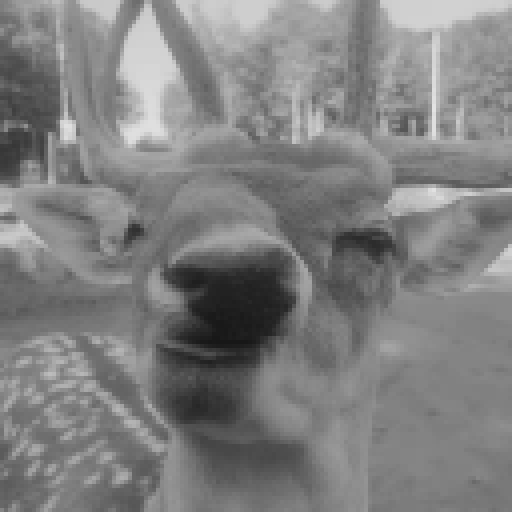
\includegraphics[scale=0.4]{./pierrelouisdiviserecursiveseuil2.png}}
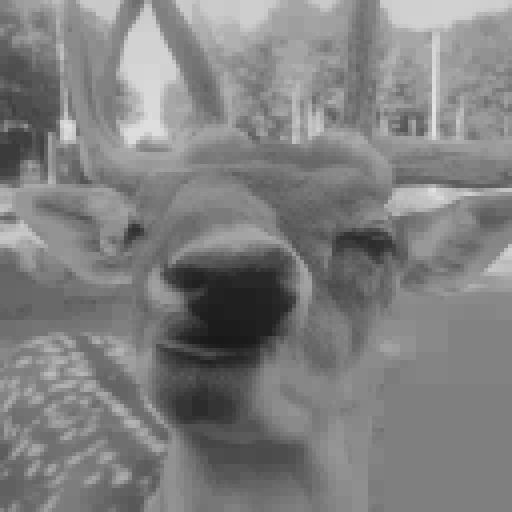
\includegraphics[scale=0.4]{./pierrelouisdiviserecursiveseuil25.png}
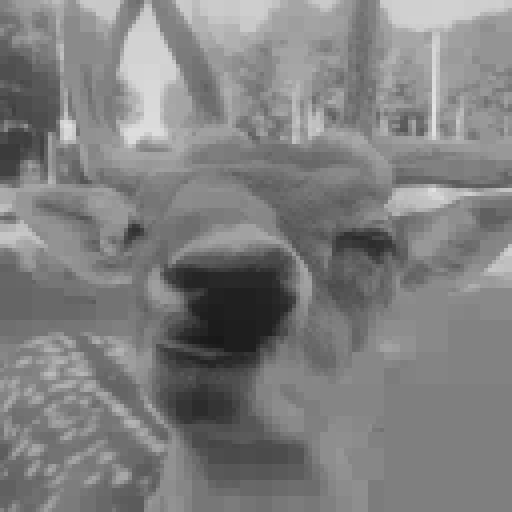
\includegraphics[scale=0.4]{./pierrelouisdiviserecursiveseuil50.png}
\caption{pierre louis avec division récursive et un seuil de 2, 25 et 50}
\end{figure}

\newpage
\section{Fusion}
Pour fusionner on créé notre graphe d'adjacence au fur et à mesure si la moyenne de 2 blocs sont proches (leur différence en valeur absolue inférieure à un seuil de fusion) alors les fusionne.
Cela pour toutes les régions voisines en prenant celle qui a la plus petite différence avec la région courante.
On a donc par rapport à précédemment plus de régions proches qui deviennent uniformes.
\begin{figure}[h]
\centerline{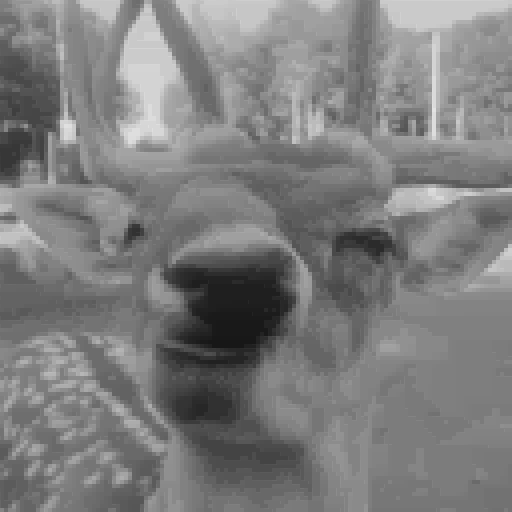
\includegraphics[scale=0.5]{./pierrelouisdiviserecursiveseuil2Fusion.png}}
\caption{pierre louis avec division récursive et un seuil de 2 et un seuil de fusion de 8}
\end{figure}

\begin{figure}[h]
\centerline{\includegraphics[scale=0.5]{./pierrelouisdiviserecursiveseuil25Fusion.png}}
\caption{pierre louis avec division récursive et un seuil de 25 et un seuil de fusion de 8}
\end{figure}

\end{document}